\section{Study Design}\label{sec:design}\label{sec:design}
% Section dedicated to document your study was carried out
This study is designed and carried out by following the guidelines on secondary studies \cite{syslit1,syslit2,syslit3}. We provide a replication package, which contains the raw data from each intermediate step executed during the search and selection phase (including any scripts that were used), over at our GitHub\footnote{\url{https://github.com/ThijmenKurk/literature-study}}.

\subsection{Research Approach}
\todo{What is the research goal of this study should be documented in this section. This can follow the GQM approach, as described in the following sentence, which NEEDS TO BE REPHRASED IN YOUR OWN WORDS if you want to include it in your study.}
\todo{In this subsection, the research questions underlying your study should be reported}

The goal of this literature study is to provide the reader with a model that contains an overview of components that are generally found inside microservice architectures. Furthermore, we describe the challenges and available solutions that are commonly used for the data management between microservices (i.e., transactions that spawn over multiple microservices). Towards our goal we have drafted the following research questions.
\begin{enumerate}
    \item[{RQ}1] How can modern microservice architectures be modelled?
    \item[    -] We drafted this research question to provide a generalizable model for modern microservice architectures derived from scientific literature. This high-level overview will facilitate the next research question by providing context, definitions, and concepts found in microservice architectures.
    \item[{RQ}2] What are the challenges and available solutions used for inter-microservice data management?
    \item[    -] We aim to identify challenges within inter-microservice data management such that we can expose the (potential lack of) available solutions.
\end{enumerate}

\subsection{Search and Selection}
\todo{How was the initial search for literature carried out should be reported in this section}
We now describe the search and selection process of this study. The study design (i.e., the search string and selection criteria) is locked in after the start of the search and selection process to avoid any personal biases. This and other threads to validity are discussed in Section \ref{sec:threats}.

\subsubsection{Initial Search}
For this study \textit{Elsevier Scopus}\footnote{\url{https://www.scopus.com/}} is used as our search engine. This tool has functionality such as the ability to, export search results to different formats (including but limited to CSV and BibTex), apply in-depth filters and search through both citations and references of studies automatically. All of which are used to facilitate the next steps. Our initial selection of 192 studies was a result of the query shown in Figure \ref{fig:search-string-refined}.


\begin{figure}
    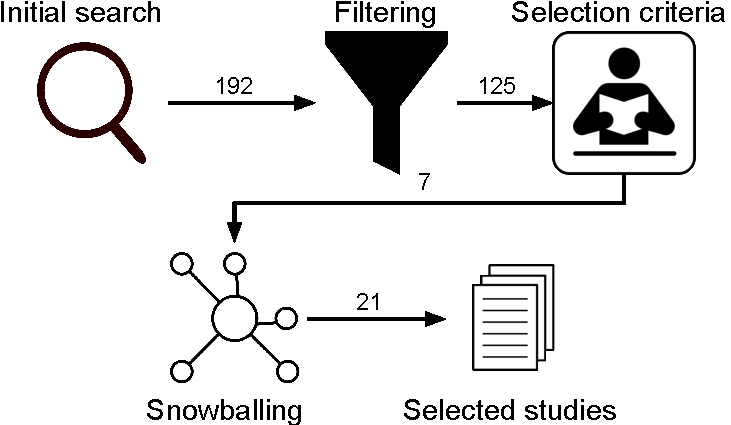
\includegraphics[scale=0.42]{images/search-and-selection.pdf}
    \caption{Search and selection process}
    \label{fig:search-and-selection}
\end{figure}

\subsubsection{Filtering}
Using the filter functionality of Scopus we were able to further refine our selection. First, all literature not pertaining to the subject area computer science is removed. Secondly, we filter the literature such that it only contains conference papers, articles and book chapters that are in a finalized state. Thirdly, we exclude any papers that are not written in English. Finally, we omit literature with the subject of microservices in combination with Internet of Things (IoT) and network architectures, since this is out of scope of this review. Refining our selection to a total of 125 studies.


\subsubsection{Application of Selection Criteria}
\todo{ In this section, the selection criteria, in terms of inclusion and inclusion criteria should be documented. See examples below, which should be adapted to your specific case and, in any case, *rephrased in our own words*}

The selected studies are manually filtered using the inclusion and exclusion criteria \cite{syslit1,syslit2,syslit3} listed below.
\begin{enumerate}
    \item[{I}1] Studies focussing on microservices or microservice architectures.
    \item[{I}2] Studies focussing on data management within microservice architectures.
    \item[{I}3] Studies that are peer-reviewed.
    \item[{I}4] Studies that are written in English.
    \item[{E}1] Studies that marginally describe a microservice architecture.
    \item[{E}2] Studies describing the migration process from a monolith to microservice architecture.
    \item[{E}3] Studies that are of bad quality (e.g., many spelling errors, unreadable sentences, etc.)
    \item[{E}4] Studies not available as full-text.
\end{enumerate}
\begin{equation}
    (I1 \vee I2) \wedge I3 \wedge I4 \wedge \neg E1  \wedge \neg E2  \wedge \neg E3  \wedge \neg E4
    \label{eq:inc_excl_criteria}
\end{equation}

The criteria are applied by following equation~\ref{eq:inc_excl_criteria} during each of the following two steps. First, we read the title and abstract of the study. Last, we read each study full-text. After the manual filtering is done we are left with a selection of 7 studies.

\subsubsection{Snowballing}
\todo{If a snowballing approach was used for the literature review, its details should be documented in this subsection}
During this phase \textit{forward} and \textit{backward} snowballing \cite{syslit4} is used on the selected studies. On completion, we expanded our selection to 21 studies.

\subsubsection{Final Selection}
The search and selection process selected 21 studies for this review. An overview of the selected studies can be found in Table~\ref{table:selected-studies}.

% \subsubsection{Exclusion during Data Extraction}
% \todo{Write about studies excluded after being read for a second time in the Data Extraction phase}

\subsection{Data Extraction}
\todo{Report in this section the data extraction followed to gather the data for the study (e.g., what process did you followed to gather the data in the companion data extraction spreadsheet?)}
During the data extraction phase, every selected study is read full-text and information pertaining to the research questions is stored in a spreadsheet. The goal of this phase it to find patterns within MSAs such that the primary components within these patterns can be described and modelled.

\subsection{Data Synthesis}
During the data synthesis phase we iteratively go through the extracted data and update our model to fit it. This method is called narrative synthesis and is commonly used when synthesizing literature in the context of systematic literature reviews \cite{popay2006guidance}. The product of this step is a generalized model of MSAs and the challenges and potential solutions within data management, both of which are described in Section~\ref{sec:results}.


% \subsection{Study Replicability}
% \todo{To ensure the replicability of the study, you should document in this section the data you make available (e.g. via Google Drive) to replicate the findings, this include:
%     * the research protocol
%     * the complete list of primary studies
%     * the parameters composing the potential classification framework you built
%     * the raw extracted data of each selection phase}